\documentclass{minimal}

\usepackage{tikz}
\usetikzlibrary{calc, arrows, fit, positioning}
\definecolor{clamped}{RGB}{200,200,200}

\begin{document}
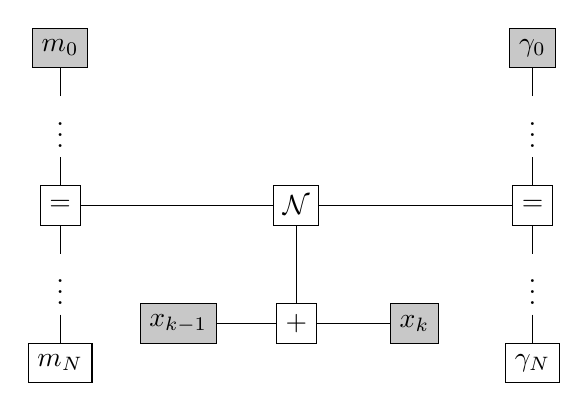
\begin{tikzpicture}
    [
        node distance=15mm,auto,>=latex',
        box/.style={draw, minimum size=.5cm},
        bbox/.style={draw, minimum size=1cm},
        blackbox/.style={draw, fill=black, minimum size=0.25cm}
    ]
    \tikzstyle{line} = [draw, -latex,>=latex]
    \tikzstyle{dash} = [dashed, -latex,>=latex]
    \tikzstyle{branch} = [fill,shape=circle,minimum size=3pt,inner sep=0pt]
    
    \begin{scope}
        \node[box] (add) {+};
        \node[box, left of=add, fill=clamped] (x_k_min) {$x_{k-1}$};
        \node[box, right of=add, fill=clamped] (x_k) {$x_{k}$};
        \node[box, above of=add] (N) {$\mathcal{N}$};
        \node[box, right of=N, node distance=3.0cm] (gam_eq) {=};
        \node[box, left of=N, node distance=3.0cm] (m_eq) {=};
        \path[line] (add) edge[-] (x_k_min);
        \path[line] (add) edge[-] (x_k);
        \path[line] (add) edge[-] (N);
        \path[line] (N) edge[-] (gam_eq);
        \path[line] (N) edge[-] (m_eq);

        \node[above of=m_eq, node distance=1.0cm] (m_above_dots) {$\vdots$};
        \node[box, above of=m_above_dots, node distance=1.0cm, fill=clamped] (m_0) {$m_0$};
        \node[below of=m_eq, node distance=1.0cm] (m_below_dots) {$\vdots$};
        \node[box, below of=m_below_dots, node distance=1.0cm] (m_N) {$m_N$};
        \path[line] (m_eq) edge[-] (m_above_dots);
        \path[line] (m_above_dots) edge[-] (m_0);
        \path[line] (m_eq) edge[-] (m_below_dots);
        \path[line] (m_below_dots) edge[-] (m_N);

        \node[above of=gam_eq, node distance=1.0cm] (gam_above_dots) {$\vdots$};
        \node[box, above of=gam_above_dots, node distance=1.0cm, fill=clamped] (gam_0) {$\gamma_0$};
        \node[below of=gam_eq, node distance=1.0cm] (gam_below_dots) {$\vdots$};
        \node[box, below of=gam_below_dots, node distance=1.0cm] (gam_N) {$\gamma_N$};
        \path[line] (gam_eq) edge[-] (gam_above_dots);
        \path[line] (gam_above_dots) edge[-] (gam_0);
        \path[line] (gam_eq) edge[-] (gam_below_dots);
        \path[line] (gam_below_dots) edge[-] (gam_N);
    \end{scope}

\end{tikzpicture}
\end{document}